%%%%%%%%%%%%%%%%%%%%%%%%%%%%%%%%%%%%%%%%%%%%%%%%%%%%%%%%%%%%%%%%%%%%%%
% How to use writeLaTeX: 
%
% You edit the source code here on the left, and the preview on the
% right shows you the result within a few seconds.
%
% Bookmark this page and share the URL with your co-authors. They can
% edit at the same time!
%
% You can upload figures, bibliographies, custom classes and
% styles using the files menu.
%
%%%%%%%%%%%%%%%%%%%%%%%%%%%%%%%%%%%%%%%%%%%%%%%%%%%%%%%%%%%%%%%%%%%%%%

\documentclass[12pt]{article}
\usepackage{amsmath,amssymb}

\usepackage{sbc-template}

\usepackage{graphicx,url}

\usepackage{indentfirst}

\usepackage[brazil]{babel}   
\usepackage[utf8]{inputenc}  

\sloppy

\title{Título}

\author{Edson Fagner da Silva Cristovam \inst{1} }

\address{Departamento de Estatística e Informática -- Universidade Federal Rural de Pernambuco\\
  Rua Dom Manuel de Medeiros, s/n, - CEP: 52171-900  -- Recife -- PE -- Brasil
  \email{fagner.cristovam@hotmail.com}
}

\begin{document} 

\maketitle

% SEÇÕES
\begin{resumo} 
  ESCREVA SEU RESUMO AQUI
  \end{resumo}

\begin{abstract}
  [do write your abstract in english, use Google Translate and do corrections]
\end{abstract}
\section{Introdução}
No seu resumo descreva sucintamente o contexto do trabalho e o que foi feito. Os tópicos a serem abordados são: 

\subsection{Contexto/Problema}
Em qual contexto seu trabalho está inserido? 
Quais lacunas são observadas nesse contexto?
Qual a motivação/justificativa do trabalho? (porque fechar essas lacunas é importante?)
 
\subsection{Objetivos}
Qual o objetivo geral do trabalho?
Quais são os objetivos específicos?

\subsection{Abordagem proposta}

\subsection{Contribuições}

\subsection{Organização do trabalho}

Como o trabalho está organizado?
\section{Referencial teórico}
\label{sec:referencialTeorico}
% Os principais conceitos aos quais os trabalho está relacionado. Por exemplo, apresentar os conceitos de Aprendizado de Máquina e métodos relacionados.
% As principais técnicas e métodos nos quais o trabalho se apoia (referências)

Antes de tratar sobre as definições mais específicas que este trabalho vai utilizar, gostaria de trazer uma definição mais geral em que o problema está incluído. Podemos compreender Sistemas de Informação como sistemas, sejam eles manuais ou automatizados, inter-relacionados que atuam armazenando, processando e transmitindo dados que representam informações para as partes interessadas (\textit{stakeholders}). De forma mais geral, esses sistemas "\textit{atuam em conjunto para o cumprimento de uma tarefa ou um objetivo}" \cite{turban2009business}. O grupo básico de operações de um Sistema de Informação é constituído pelas entradas, pelo processamento e pelas saídas (Figura \ref{fig:operacoesBasicaSistemas}). A entrada é o conjunto de dados que será usado pelo sistema, o processamento é composto pela transformações e combinações que os dados de entradas serão submetidos e, por fim, a saída é o produto obtido por meio do processamento dos dados de entrada. Em alguns casos, o sistema pode ser retroalimentado (\textit{feedback}), fazendo com que os dados de saída sejam manipulados como dados de entrada em uma nova execução. Neste processo, também é comum que ocorra o armazenamento dos dados de entrada e de saída para serem utilizados posteriormente, como pode ser visto na Figura \ref{fig:operacoesBasicaSistemas}.

\begin{figure}[ht]
\centering
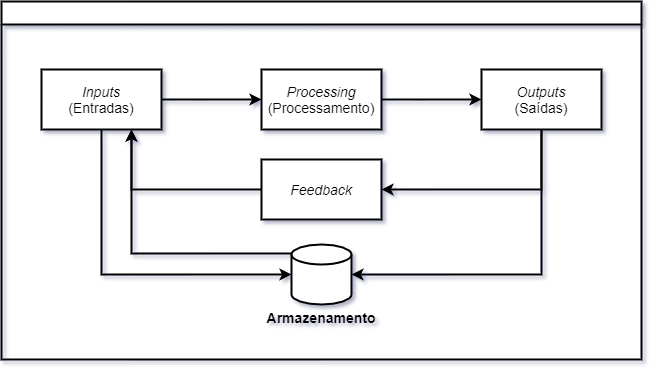
\includegraphics[width=1\textwidth]{imagens/operacoes-basicas-sistema-informacao.png}
\caption{Operações básicas de um Sitema de Informação.}
\label{fig:operacoesBasicaSistemas}
\end{figure}

% TODO falar sobre informação e dados https://integrada.minhabiblioteca.com.br/reader/books/9786556901916/pageid/17


\section{Ferramentas Utilizadas}
\label{sec:ferramentas}
Discorrer sobre as ferramentas que são utilizadas para efetuar o trabalho.

\subsection{Python}
\label{subsec:python}
Python é uma linguagem de programação desenvolvida no final dos anos 80. Ela foi concebida pelo matemático holandês, Guido van Rossum, que a criou quando sentiu a necessidade de uma linguagem mais simples de se trabalhar que a C e que não tivesse as limitações do \textit{shell script}, linguagem de comando utilizada por ele \cite{de2020python}. Segundo pesquisa do Stack Overflow, um site de perguntas e respostas para programadores, Python é a terceira linguagem mais popular na plataforma \cite{stackoverflow:survey}. Ela é bastante conhecida no seu uso em automação de tarefas, desenvolvimento web e aprendizado de máquina devido à sua sintaxe sucinta e breviloquente \cite{de2020python}.

Python é uma linguagem de alto nível, isto significa que, teoricamente, ela está mais próxima da linguagem natural que da linguagem de máquina. Também é uma linguagem interpretada, na qual o código fonte é convertido para o formato intermediário chamado de \textit{bytecode} e o interpretador fica responsável por converter o \textit{bytecode} para o formato próprio para ser executado no sistema operacional desejado. Python é uma linguagem de programação multiparadigma, que se encaixa em muitos paradigmas como o imperativo e funcional. A tipagem do Python é dinâmica, pois a linguagem determina o tipo de dado de uma variável baseada no valor que essa variável armazenará, não havendo necessidade de declarar o tipo explicitamente \cite{de2020python}.


\subsection{Amazon Web Services}
\label{subsec:aws}

% https://aws.amazon.com/pt/
% https://aws.amazon.com/pt/what-is-aws/?nc1=f_cc

Amazon Web Services, ou simplesmente AWS, é a plataforma de nuvem da Amazon que disponibiliza mais de 200 serviços de \textit{datacenters} ao redor do globo. A plataforma oferece infraestrutura em nuvem como computação, armazenamento de arquivos ou em banco de dados, criptografia, ferramentas de \textit{machine learning}, \textit{data lakes} e \textit{internet} das coisas, além de suporte ao Docker e às linguagens de programação: .NET, Python, Java, JavaScript e PHP. A AWS dispõe de uma infraestrutura que satisfaz requisitos de segurança militares, compatível com 90 normas de segurança e certificações. Sua rede oferece alta redundância e taxa de transferência com baixa latência, estando presente em 81 zonas de disponibilidade que estão distribuídas em 25 regiões geográficas ao redor de globo \cite{aws:about}.

\subsubsection{AWS Athena}
\label{subsec:athena}
% https://aws.amazon.com/pt/athena/

O AWS Athena, ou somente Athena, é um serviço de consultas de dados \textit{serverless}, isto é, que segue um modelo de execução de computação em nuvem alocando recursos de processamento sob demanda e que elimina a necessidade do usuário de gerenciar a infraestrutura do servidor. O serviço é baseado no \textit{software} de código aberto chamado Presto, da The Presto Foundation, ele usa o padrão SQL (\textit{Structured Query Language} ou Linguagem de Consulta Estruturada) para acessar os dados dos arquivos que ficam armazenados no Amazon S3 (Seção \ref{subsec:s3}). É possível configurar o Athena para que ele trate um ou mais conjuntos de arquivos de forma análoga ao modelo relacional, estruturando-os em forma de tabelas e atribuindo tipos para as colunas, isso graças a sua integração com o AWS Glue Data Catalog. O AWS Athena tem suporte para arquivos organizados em linhas como CSV, Avro e JSON e os formatos colunares ORC e Parquet \cite{aws:athena}.

\subsubsection{Amazon S3}
\label{subsec:s3}
% https://aws.amazon.com/pt/s3/

Amazon Simple Storage Service (Amazon S3) é um serviço da AWS para armazenamento de arquivos de forma escalável. Os dados armazenados no S3 podem ser usados em diversos casos de uso como \textit{data lakes}, \textit{sites} e aplicações móveis. O serviço também oferece suporte à criptografia e ao gerenciamento de autorizações, permitindo que a organização administre o nível de acesso dos seus colaboradores. Ele fornece uma durabilidade para os arquivos de 99,99\%, pois realiza cópias automáticas de todos os documentos e os conserva em diversas regiões, aumentando sua disponibilidade e protegendo-os contra erros ou falhas \cite{aws:s3}.


\subsection{MongoDB}
\label{subsec:mongo}
% https://www.mongodb.com/
O MongoDB é um \textit{software} de banco de dados orientado a documentos com o código aberto, sendo classificado como um NoSQL, também conhecido como \textit{Not only SQL} (Não somente SQL) – um termo usado para categorizar bancos de dados não relacionais, isto é, uma classe de bancos de dados que armazena e recupera as informações que são estruturadas de uma maneira diferente a da abordagem com relações tabulares. Ele é escrito na linguagem C++ e é distribuído em múltiplas plataformas. A organização dos documentos é feita em um formato similar ao JSON, em uma disposição composta por um par de campo e valor, em que os valores dos campos podem conter dados de tipos primitivos, outros documentos ou vetores, o que fornece a possibilidade de se criar hierarquias complexas que podem ser indexadas, o que facilita a recuperação das informações. Os documentos são agrupados em coleções, uma perspectiva análoga as tabelas do modelo relacional \cite{mongoDB2021}.

O MongoDB apresenta suporte a buscas por campo, intervalo de valor, expressões regulares e também por funções JavaScript personalizadas \cite{mongoDB2021}. As agregações de dados do MongoDB podem ser feitas usando um \textit{pipeline} de agregação ou com o \textit{map-reduce}, que está depreciado e possui um desempenho pior que o do \textit{pipeline} \cite{mongoDBagregacao}. Além disso, ele é capaz de executar transção ACID – acrônimo em inglês para: \textit{Atomicity}, \textit{Consistency}, \textit{Isolation}, \textit{Durability}, ou em uma tradução livre, Atomicidade, Consistência, Isolamento e Durabilidade — que é um conjunto de propriedades para as transações em banco de dados \cite{mongoDBACID}.


\subsection{PostgreSQL}
\label{subsec:postgres}
% https://www.postgresql.org/
% https://pt.wikipedia.org/wiki/PostgreSQL
Falar sobre PostgresSQL...

\section{Abordagem proposta}
\label{sec:abordagem}
% Nessa seção devem ser apresentados os métodos utilizados no trabalho, ferramentas, dados e materiais.

Empresas que atuam em uma grande área do território nacional atendendo a um grande número de clientes podem ser ré de diversas ações judiciais iniciadas pelos consumidores que se sentiram lesados com os serviços prestados. Desse modo, essas numerosas ações judiciais podem ocorrer em diferentes locais ou comarcas, \enquote{\textit{território em que o juiz de primeiro grau irá exercer sua jurisdição e pode abranger um ou mais municípios}} \cite{cnj:comarca}, o que dificulta o acompanhamento dos processos forenses. Assim sendo, manter uma equipe jurídica do tamanho necessário para cuidar dessa volumosa soma de processos, manualmente, pode ser muito custoso para a empresa, sendo capaz de prejudicar o bem-estar financeiro e jurídico dela.

Diante desse cenário, surgiram empresas que ofertam \enquote{inteligência jurídica}, acompanhando os inúmeros processos jurídicos por meio da sua coleta, armazenando-os em um banco de dados. Esses dados processuais são disponibilizados pelos sistemas de justiça providenciados por meio das suas plataformas digitais como o Projudi do TJPE \cite{tjpe} e o e-SAJ CE \cite{esajce}. Essa coleta otimiza o trabalho das equipes jurídicas das empresas, no entanto, esses dados podem ser usados para fornecer muito mais informações para o setor jurídico da empresa e até contribuir para o seu \textit{business intelligence} (BI), revelando novas perspectivas que servirão de base para a tomada de decisão.

Mas no Brasil existem diversas plataformas digitais de justiça, em que cada uma disponibiliza os dados à sua maneira. Essa diferenciação na representação de um mesmo tipo de informação é uma problema quando se deseja usar técnicas de \textit{business intelligence} por meio de um \textit{data warehouse} (Seção \ref{subsec:datawarehouse}), pois sem um tratamento prévio, o agrupamento dos dados nessa situação não apresenta resultados satisfatórios. Então é necessário utilizar alguma estratégia para padronizar esses dados, sendo o ETL (Seção \ref{subsec:etl}) uma das técnicas mais utilizadas para tal.


\subsection{Processos}
\label{subsec:processos}

Os elementos contidos no processo são imprescindíveis para a construção do \textit{data warehouse} focado na obtenção de conhecimento jurídico e na aplicação da jurimetria, isto é, \enquote{\textit{a estatística aplicada ao Direito}} \cite{newlawJurimetria}.

Os principais dados de um processo judicial, mas não se limitando somente a eles, são a sua Numeração Processual Única (NPU) ou somente número, as partes envolvidas, os andamentos ou movimentações e a fonte.

A NPU é composta por vinte dígitos e foi instituída pelo Conselho Nacional de Justiça (CNJ) com o intuito de facilitar a consulta das informações referente a um processo, pois os números dos processos mudavam frequentemente em cada instância ou recurso. A Numeração Processual Única vale para os tribunais de todo o país e apresentam a seguinte estrutura \enquote{NNNNNNN-DD.AAAA.J.TR.OOOO} no qual \cite{jusbrasilNPU}:

\begin{itemize}
    \item \textbf{NNNNNNN-DD}: representam o número sequencial do processo e seu dígito verificador \cite{TRF4NPU}.
    \item \textbf{AAAA}: diz respeito ao ano de avaliação do processo \cite{TRF4NPU}.
    \item \textbf{J}: informa qual o órgão ou segmento do Poder Judiciário que o processo pertence \cite{TRF4NPU}.
    \item \textbf{TR}: indica o tribunal do respectivo segmento ou circunscrição judiciária \cite{TRF4NPU}.
    \item \textbf{OOOO}: remete à unidade de origem do processo \cite{TRF4NPU}.
\end{itemize}

As partes do processo são compostas pelo autor, que desempenha o papel de polo ativo do processo, ou seja, aquele que recorre à tutela jurídica do estado, tomando a posição ativa, e pelo réu, que realiza o papel do polo passivo, estando sujeito à ação processual iniciada pelo autor.

As movimentações de um processo são um conjunto de informações que comunicam a evolução processual ao longo da tramitação judicial. Elas podem conter os mais diferentes tipos de conhecimentos a respeito do processo, como os informes sobre o dia de uma audiência, notificação de emissão de intimação ou até mesmo a notícia da sentença do juiz. Nesse sentido, é usando as informações dos andamentos que o ETL fará a maior parte do seu processamento. As movimentações podem ser compostas pelos seguintes campos: 

\begin{itemize}
    \item \textbf{Título}: informa o assunto que o andamento trata.
    \item \textbf{Texto}: corpo do texto (opcional).
    \item \textbf{Complemento}: informações complementares (opcional)
    \item \textbf{Data}: dia e hora que o andamento foi disponibilizado no sistema de justiça.
\end{itemize}

Por fim, a fonte informa de maneira explícita em qual sistema o processo foi extraído. Essa informação é útil para definir quais rotinas serão aplicadas na etapa de transformação (Seção \ref{subsec:transformacao}) do ETL.


\subsection{ETL para Jurimetria}
\label{subsec:jurimetria}

A técnica de ETL usada neste trabalho segue o modelo de \textit{pipeline}, no qual cada uma das etapas do fluxo de trabalho possuem uma tarefa muito bem estabelecida e são conectadas em série (Figura \ref{fig:stepsFlow}). Cada nó dessa fila é uma estrutura que recebe o nome de \textit{step}.

\begin{figure}[ht]
\centering
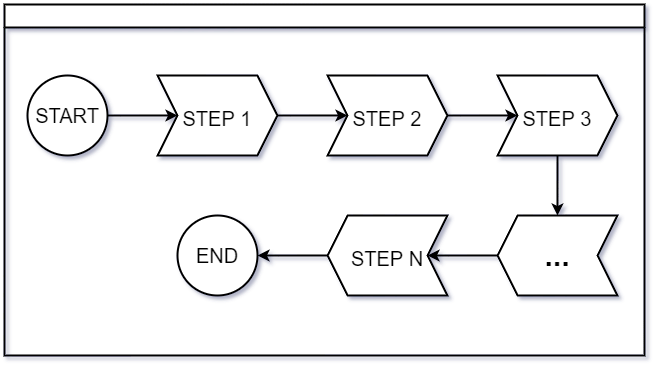
\includegraphics[width=1\textwidth]{imagens/steps-flow.png}
\caption{Fluxo de execução dos \textit{steps}.}
\label{fig:stepsFlow}
\end{figure}

O \textit{step} é um conjunto de operações que serão aplicadas ao processo para realizar um objetivo bem definido. No projeto, ele é codificado como uma classe Python (Seção \ref{subsec:python}) com um método obrigatório chamado \textit{transform}. O \textit{transform} é a função que receberá o processo e aplicará as inferências e transformações necessárias para alcançar o seu objetivo.

Os processos são extraídos dos vários sistemas jurídicos pela equipe de extração e armazenados como documentos em um banco de dados MongoDB (Seção \ref{subsec:mongo}). Esses documentos serão usados no processamento do ETL, podendo ser combinados com informações complementares fornecidas pela empresa, que preparará os dados e também criará novos para serem inseridos no \textit{data warehouse}. No ETL, os documentos são lidos do MongoDB e estruturados como um dicionário do Python (Figura \ref{fig:processoPython}).

\begin{figure}[ht]
\centering
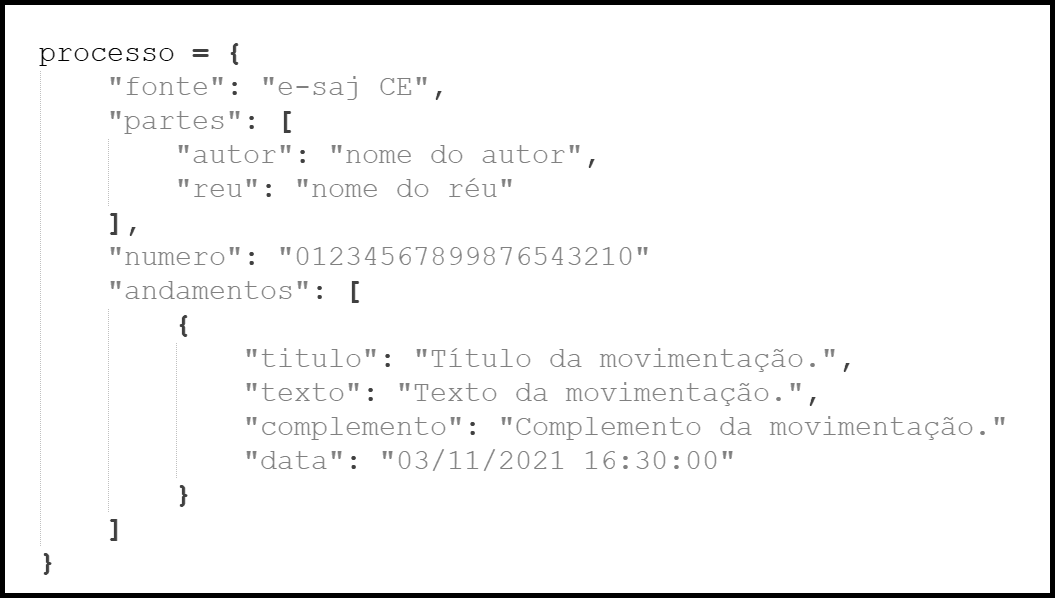
\includegraphics[width=1\textwidth]{imagens/processo-python.png}
\caption{Exemplo de um processo como um dicionário do Python.}
\label{fig:processoPython}
\end{figure}


\subsubsection{Steps}
\label{subsec:steps}

Para esse trabalho, não serão abordados todos os \textit{steps} que são efetivamente realizados pela empresa, mas somente um recorte de alguns deles. Com exceção do primeiro \textit{step}, que trata da normalização dos dados, cada um dos demais \textit{steps} são responsáveis por adicionar mais um campo na raiz do dicionário que representa o processo (Figura \ref{fig:processoInStep}). Normalmente esse campo tem o nome do próprio \textit{step} que o gerou e seu valor é uma lista de dicionários. Esses novos campos darão origem às tabelas no banco de dados final, em que o nome da tabela será o nome do próprio campo, as suas colunas serão as chaves dos dicionários que estão na lista e os valores que popularão a tabela serão os valores dos dicionários em que a chave corresponda ao nome da coluna (Figura \ref{fig:processoParaTabela}).

\begin{figure}[ht]
\centering
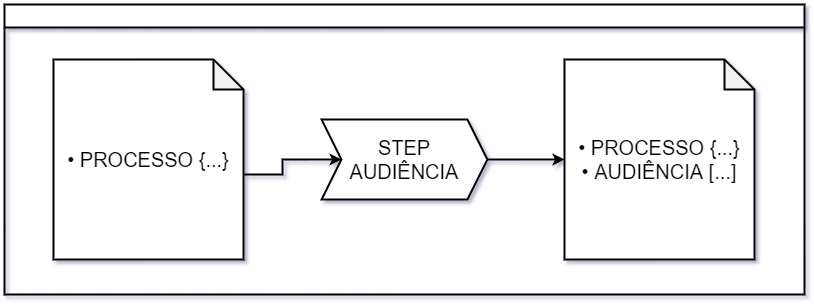
\includegraphics[width=1\textwidth]{imagens/processo-in-step.png}
\caption{Exemplo de \textit{step} enriquecendo o documento (processo) com novas informações.}
\label{fig:processoInStep}
\end{figure}

\begin{figure}[ht]
\centering
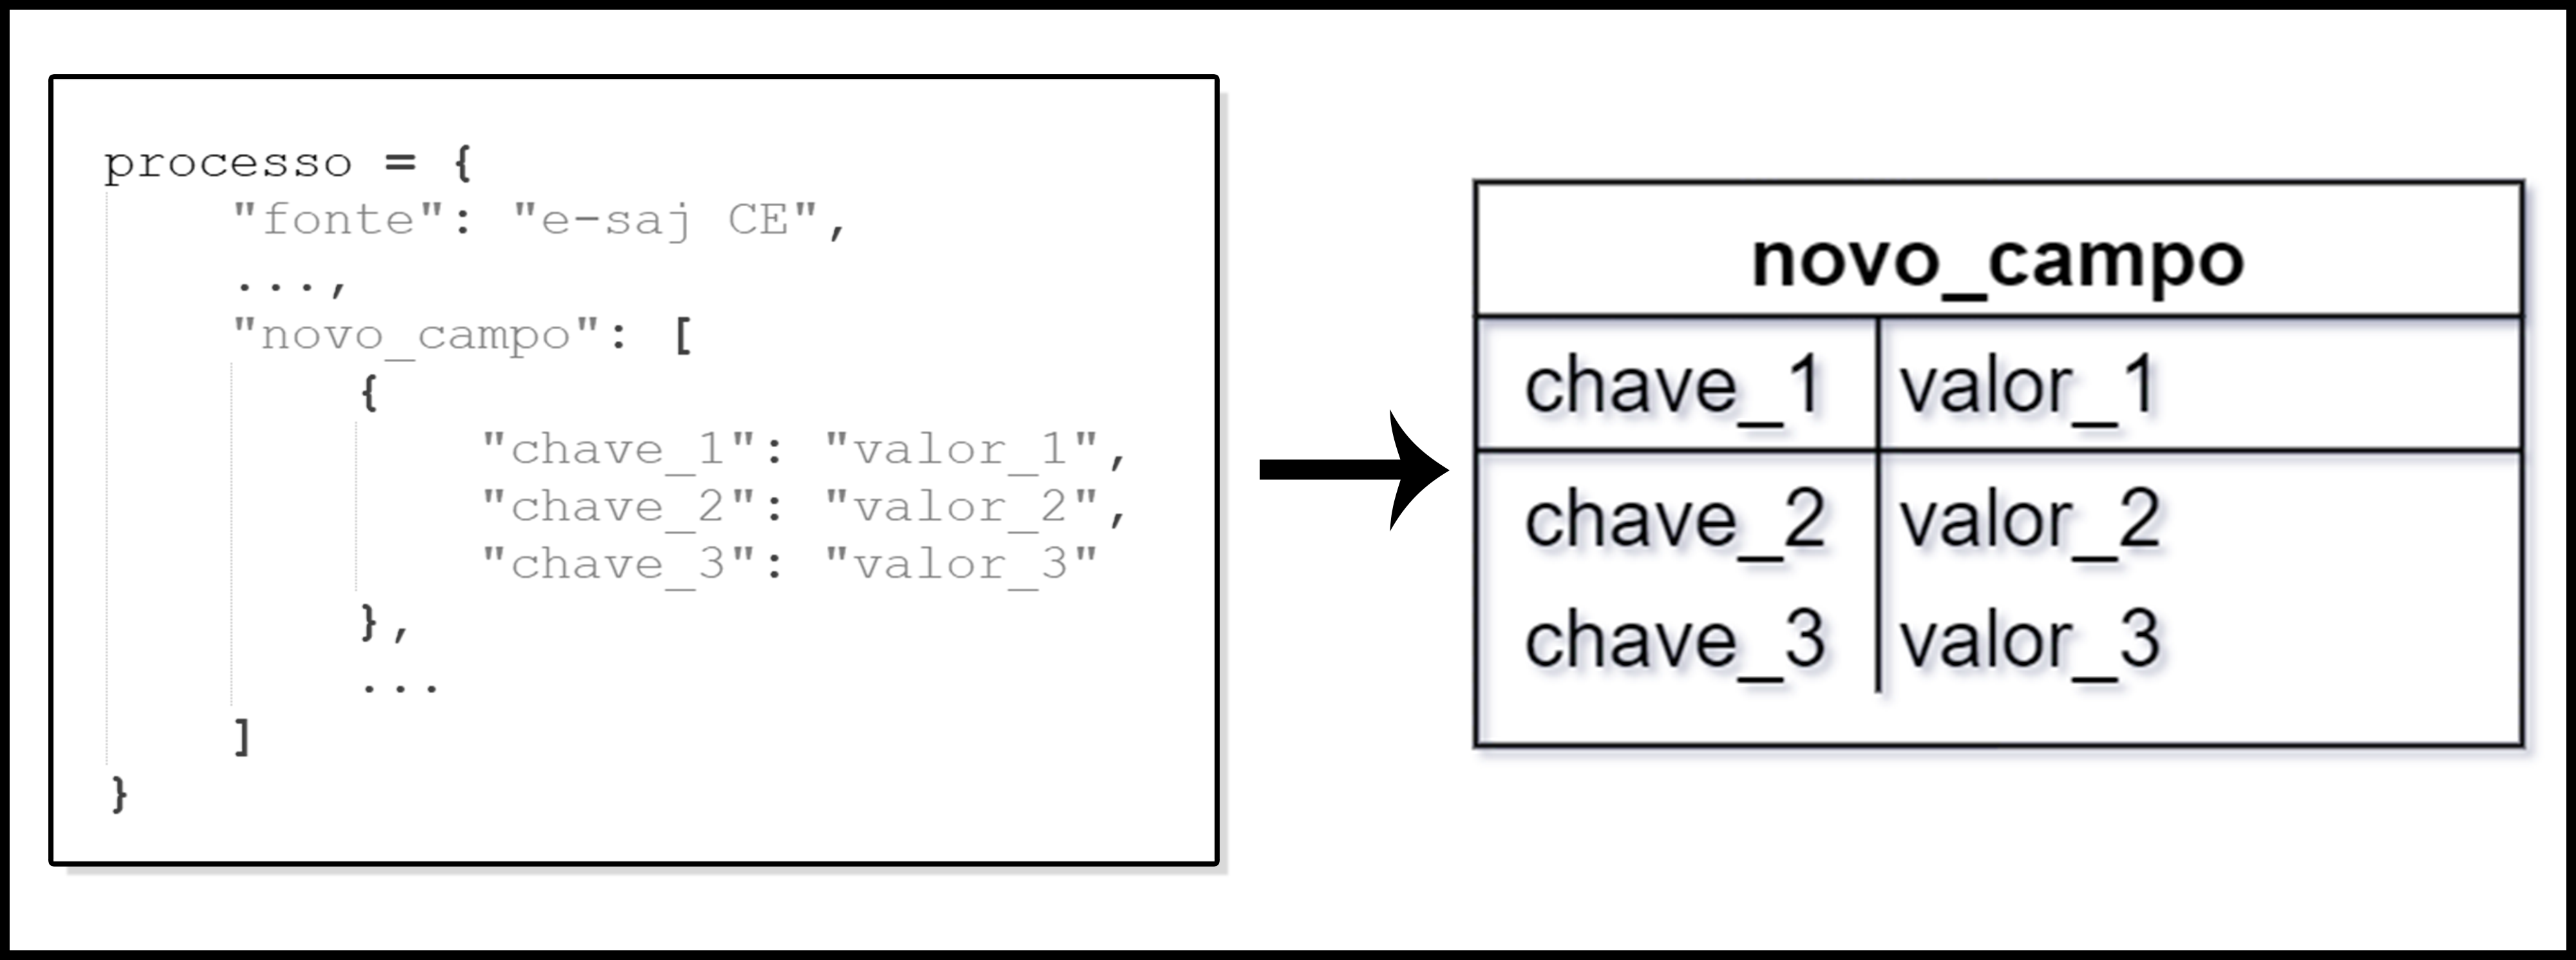
\includegraphics[width=1\textwidth]{imagens/processo-para-tabela.png}
\caption{Conversão de novo campo inserido por um \textit{step} em tabela.}
\label{fig:processoParaTabela}
\end{figure}

O primeiro \textit{step}, chamado de \enquote{\textit{ProcessoClean}}, é o responsável pela normalização dos dados de um processo por meio de diversas conversões e substituições. Esse passo é necessário, pois as diversas informações que estão no processo são representadas como o tipo de dado \textit{string}, o que tornaria algumas das comparações difíceis e menos diretas, e por serem capturadas de diversos sistemas, um mesmo tipo de informação pode não seguir um mesmo padrão. Além disso, alguns campos de textos podem estar mal formatados e conter caracteres especiais que aumentam a complexidade das buscas necessárias para o enriquecimento dos dados. Os principais casos que esse \textit{step} trata são os tipos numéricos, as datas e os textos.

As \textit{strings} que representam algum tipo numérico como inteiros (\textit{integer}) ou números de ponto flutuante (\textit{float}) devem ser convertidas para os seus respectivos tipos, pois somente dessa forma as agregações realizadas pelo \textit{data warehouse}, como somas e médias, podem ser executadas corretamente. Para esse fim, as expressões regulares, ou \enquote{regex} (abreviação do inglês \textit{regular expression}), são uma ótima ferramenta na preparação desses textos para serem transformados, porque conseguem representar uma infinidade de padrões de maneira bem simples. Expressões como \enquote{[0-9]+} ou \enquote{\textbackslash d+} representam uma cadeia de números com 1 ou mais dígitos. Com isso, se torna muito simples a remoção de qualquer \enquote{impureza}, ou seja, tudo aquilo que não exprime um número, antes de modificar a \textit{string} para \textit{interger} ou \textit{float}.

As datas também precisam passar do formato de texto para um que reflita melhor as suas características e facilite a execução dos passos em que elas são essenciais. No nosso caso, o formato para o qual as datas em formato \textit{string} serão convertidas será o \textit{datetime} da linguagem Python e o \textit{timestamp} quando forem inseridas no banco de dados final. Com ele é possível realizar facilmente diversas operações que seriam muito mais difíceis de serem executadas sobre \textit{strings} e também padronizamos as várias formas que as datas podem apresentar (Ex: \enquote{03/11/2021}, \enquote{03-11-2021} e \enquote{2021.11.03}). Com o \textit{datetime} é possível comparar se uma data é maior que outra sem erros, ser maior significa que uma data é posterior a outra. Em um exemplo simples, colacionando duas datas em padrão de texto, em que a primeira data é \enquote{10/11/2021} e a segunda \enquote{11/10/2021}, se efetuarmos a operação de maior que entre a primeira e segunda data, obteremos o resultado falso, porque esse tipo de operação entre \textit{strings} é feita comparando carácter a carácter, porém, a primeira data é posterior a segunda, em outras palavras, o resultado esperado é verdadeiro. Além de tudo, outras operações como verificar a distância (número de dias) entre datas se torna impraticável quando elas são \textit{strings}.

E por último, será executada a normalização dos textos que já estão na tipagem correta (\textit{string}). A finalidade dessa etapa é alterar o conteúdo de modo a facilitar a pesquisa de informações sobre ele, eliminando tudo aquilo que for desnecessário e simplificando algumas informações. Inicialmente serão substituídos todos os espaços múltiplos (mais de um espaço em sequência) e outros espaçamentos especiais como tabulação, quebra de linha, quebra de página, etc, por um espaço simples. Isso facilita no momento de definir alguns padrões de busca com múltiplos termos como \enquote{decreto a sentença conforme descrito no artigo XX\dots}, tornando a escrita de uma busca exata ou de uma pesquisa com regex muito mais descomplicada. Outra padronização feita com o mesmo objetivo da transformação dos espaços extras e especiais é uniformização da \enquote{caixa das letras} dos textos, deixando todas em caixa alta ou caixa baixa, isso é feito, pois não é verdadeiro o resultado da comparação entre uma mesma letra maiúscula e minúscula. O efeito negativo que isso causa nas pesquisas pode ser exemplificado com a busca do termo \enquote{juntada de protocolo} no trecho \enquote{Juntada de protocolo de petição: cumprido em 01/05/2020.}, em que o termo não seria encontrado, visto que a letra \enquote{J} da palavra \enquote{Juntada} está em caixa diferente em ambos os textos. Existe um tratamento \enquote{especial} que deve ser feito com os textos em português também com o objetivo de facilitar as buscas. Refere-se à substituição das vogais acentuadas, como \enquote{à} e \enquote{é}, e da letra \enquote{cê-cedilha} pelos seus equivalentes na tabela ASCII (\textit{American Standard Code for Information Interchange}). O problema que a não substituição dessas letras gera é semelhante ao que ocorre com a comparação entre letras em caixas diferentes.

Os demais \textit{steps} não fazem alterações nos dados presentes no processo, mas adicionam novas informações com base em inferências feitas sobre os dados já presentes. De forma geral, as investigações executadas em cima dos dados são efetuadas usando três técnicas: uma pesquisa exata do termo, busca de padrão usando regex e o rastreio de expressões utilizando busca \textit{fuzzy}, que são buscas focadas em encontrar correspondências por aproximação, ao invés de exatidão. Com base nos resultados obtidos dessas investigações, cada \textit{step} pode introduzir novas informações ao processo, que juntamente com ele, servirá como entrada para o \textit{step} seguinte.

Finalmente, após todos os processos passarem pelos \textit{steps}, os dados serão armazenados em formato JSON no Amazon S3 (Seção \ref{subsec:s3}). Em seguida, o Athena (Seção \ref{subsec:athena}) é utilizado para estruturar esses dados que estão em JSON como tabelas de um modelo relacional a partir de arquivos no formato CSV (\textit{Comma Separated Values}) que o próprio Athena criará. Depois disso, esses arquivos CSV são utilizados para exportar as informações para o banco de dados PostgreSQL (Seção \ref{subsec:postgres}), sendo esse o formato final pré \textit{data warehouse}. Por mais contra contra-intuitivo que isso pareça, exportar o dados diretamente do Python para o PostgreSQL oferecia um desempenho bastante abaixo do que a abordagem supracitada, isso porque a maneira mais rápida de se carregar dados no PostgreSQL é utilizando CSV, exceto por usar dados em formato binário, o que diminuiu drasticamente o tempo de carga. Concluído o armazenamento no PostgreSQL, os dados estão prontos para serem carregados em qualquer sistema ou serviços de análise de negócios como o Power Bi da Microsoft ou o Google Data Studio.
\section{Conclusões}
\label{sec:conclusao}
% Relembrar qual era o objetivo do trabalho.
% Quais resultados foram alcançados?
% Quais conclusões podemos tirar a partir dos resultados?
% Quais os trabalhos futuros?

Lidar com um imenso volume de dados é um problema muito comum para as empresas na \enquote{era do \textit{Big Data}}. Ainda nesse sentido, a tendência é que essas informações cresçam cada vez mais à medida que mais e mais sistemas são informatizados. Hoje, essa conjuntura já está presente na área jurídica.

Para tratar dessas questões, a estratégia da jurimetria aplicada em um \textit{data warehouse} se mostra bastante eficaz para superar essa enorme massa de dados, usando-os para extrair informações e novas perspectivas a respeito do ambiente em que se está inserido.

No entanto, uma etapa anterior ao \textit{data warehouse}, definida em três passos, é essencial para o seu êxito: a extração, a transformação e a carga desses dados deve padronizar e estruturar toda a porção de dados que irá compor o \textit{data warehouse}.

Dessa maneira, esse aglomerado de dados se torna valioso para o negócio, mostrando para a empresa seus pontos fortes e fracos, nesse caso no âmbito jurídico, guiando as suas ações para as áreas que necessitam de sua atenção e podendo contribuir com a antecipação de problemas futuros por meio de uma abordagem estatística.

Atualmente, a maior parte dos dados que são utilizados pelo projeto percorrem um longo caminho até o seu destino. Eles transitam desde o MongoDB, passando pelo processamento do Python e pela reestruturação do Athena, até desembocar no PostgreSQL. No entanto, o Athena é uma ferramenta \enquote{poderosa} o suficiente para realizar todas as operações necessárias para aplicar o ETL sobre o conjunto de dados, dispô-los em um formato colunar, como o Apache Parquet ou \textit{Optimized Row Columnar} (ORC), que são formatos mais rápidos para a pesquisa quando comparados aos formatos em linha, e, finalmente, servir como um banco de dados fim que fornecerá as informações que serão carregadas no \textit{data warehouse}. Destarte, essa seria uma ótima atualização para ser feita no futuro por diminuir o tempo de processamento total e por simplificar a metodologia empregada, já que diminuiria o número de sistemas que precisariam de manutenção.

% TODO
% Introdução - Contexto: Falar com Rômero sobre os problemas que os clientes buscam resolver.
% GERAL: Falar com a professora Roberta sobre o trabalho e pedir sugestões e indicação de uma livro sobre ETL.

% Referências
% As referências são inseridas no arquivo  sbc-template.bib. Neste arquivo estão descritos os tipos mais comuns de referência.

Para citar referência use \cite{knuth:84}, \cite{boulic:91},  and \cite{smith:99}.

\bibliographystyle{sbc}
\bibliography{sbc-template}

\end{document}
